% fig_87b_mg_topology.tex
% TR-41: IBR microgrid busbar topology showing 87B-A and 87B-B zones
%
% Two busbars (Bus A and Bus B) connected by bus-coupler BC
% Each bus has 2 IBR feeders
% 87B-A zone covers Bus A feeders + BC from A side
% 87B-B zone covers Bus B feeders + BC from B side

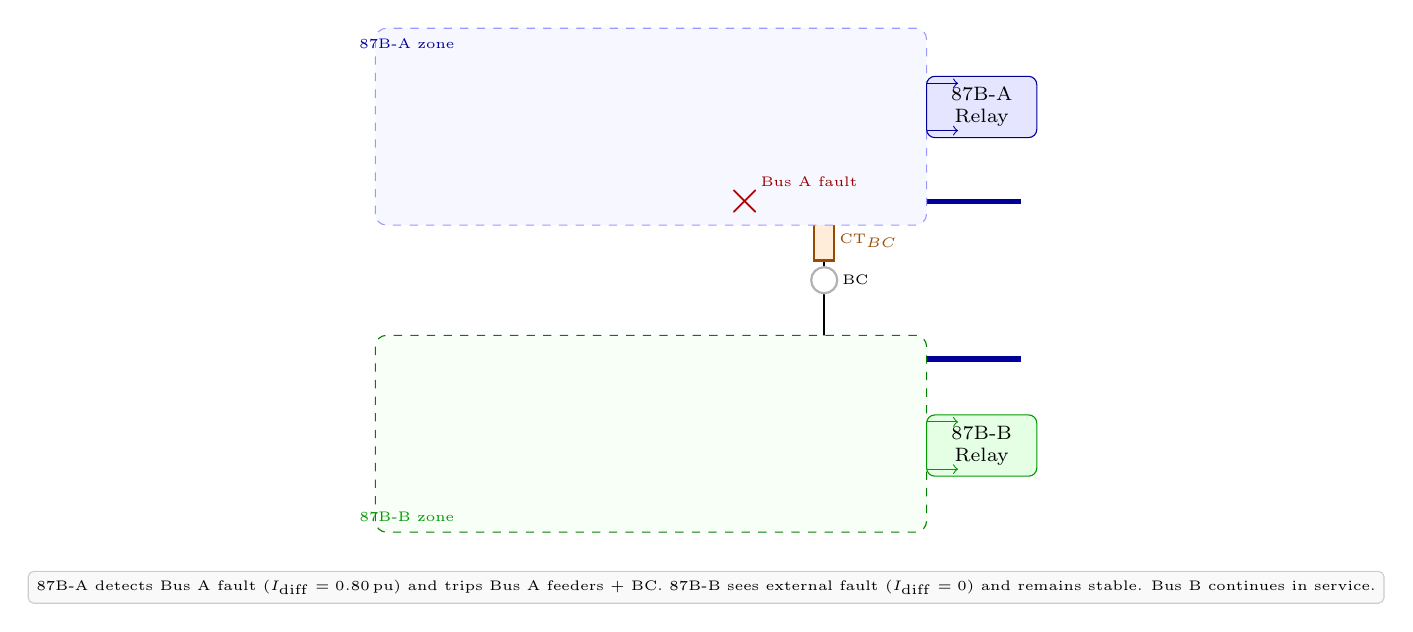
\begin{tikzpicture}[
  every node/.style={font=\small},
  ibr/.style={draw=green!60!black, thick, rectangle, rounded corners=3pt,
              fill=green!10, minimum width=1.4cm, minimum height=0.6cm,
              font=\scriptsize, align=center},
  bus/.style={draw=blue!60!black, very thick, line width=2pt},
  cb/.style={draw=gray!60, thick, circle, minimum size=0.3cm, fill=white},
  ct/.style={draw=orange!60!black, thick, rectangle, minimum width=0.25cm,
             minimum height=0.5cm, fill=orange!15},
  zone/.style={draw, dashed, rounded corners=4pt, inner sep=6pt},
]

%% ── Bus A (top) ──────────────────────────────────────────────────────────────
\draw[bus] (0, 3) -- (8, 3);
\node[blue!60!black, font=\small\bfseries, above] at (4, 3.05) {Bus A};

%% Feeder A1
\draw[thick] (1.5, 3) -- (1.5, 4.5);
\node[ct] at (1.5, 3.7) {};
\node[ibr] at (1.5, 4.8) {IBR A1};
\node[orange!60!black, font=\tiny, right=2pt] at (1.5, 3.7) {CT$_{A1}$};

%% Feeder A2
\draw[thick] (3.0, 3) -- (3.0, 4.5);
\node[ct] at (3.0, 3.7) {};
\node[ibr] at (3.0, 4.8) {IBR A2};
\node[orange!60!black, font=\tiny, right=2pt] at (3.0, 3.7) {CT$_{A2}$};

%% Bus-coupler (BC) — between buses
\draw[thick] (5.5, 3) -- (5.5, 1.5) -- (5.5, 1.0);
\node[cb] at (5.5, 2.0) {};
\node[ct] at (5.5, 2.5) {};
\node[font=\tiny, right=3pt] at (5.5, 2.0) {BC};
\node[orange!60!black, font=\tiny, right=2pt] at (5.5, 2.5) {CT$_{BC}$};

%% ── Bus B (bottom) ────────────────────────────────────────────────────────────
\draw[bus] (0, 1) -- (8, 1);
\node[blue!60!black, font=\small\bfseries, below] at (4, 0.95) {Bus B};

%% Feeder B1
\draw[thick] (1.5, 1) -- (1.5, -0.5);
\node[ct] at (1.5, 0.3) {};
\node[ibr] at (1.5, -0.8) {IBR B1};
\node[orange!60!black, font=\tiny, right=2pt] at (1.5, 0.3) {CT$_{B1}$};

%% Feeder B2
\draw[thick] (3.0, 1) -- (3.0, -0.5);
\node[ct] at (3.0, 0.3) {};
\node[ibr] at (3.0, -0.8) {IBR B2};
\node[orange!60!black, font=\tiny, right=2pt] at (3.0, 0.3) {CT$_{B2}$};

%% ── 87B relay zones ───────────────────────────────────────────────────────────
%% 87B-A zone (Bus A + upper BC CT)
\draw[zone, blue!40, fill=blue!3]
  (-0.2, 2.7) rectangle (6.8, 5.2);
\node[blue!60!black, font=\tiny, align=left] at (0.2, 5.0)
  {87B-A zone};

%% 87B-B zone (Bus B + lower BC CT)
\draw[zone, green!50!black, fill=green!3]
  (-0.2, -1.2) rectangle (6.8, 1.3);
\node[green!60!black, font=\tiny, align=left] at (0.2, -1.0)
  {87B-B zone};

%% ── 87B relay boxes ───────────────────────────────────────────────────────────
\node[draw=blue!60!black, fill=blue!10, rounded corners=3pt,
      font=\scriptsize, inner sep=4pt, minimum width=1.4cm, align=center]
  at (7.5, 4.2) {87B-A\\Relay};
\draw[->, blue!60!black, thin] (6.8, 4.5) -- (7.2, 4.5);
\draw[->, blue!60!black, thin] (6.8, 3.9) -- (7.2, 3.9);

\node[draw=green!60!black, fill=green!10, rounded corners=3pt,
      font=\scriptsize, inner sep=4pt, minimum width=1.4cm, align=center]
  at (7.5, -0.1) {87B-B\\Relay};
\draw[->, green!60!black, thin] (6.8, 0.2) -- (7.2, 0.2);
\draw[->, green!60!black, thin] (6.8, -0.4) -- (7.2, -0.4);

%% ── Fault marker ──────────────────────────────────────────────────────────────
\node[red!70!black, font=\LARGE] at (4.5, 3.0) {$\times$};
\node[red!60!black, font=\tiny, above right=2pt] at (4.5, 3.0) {Bus A fault};

%% ── Caption annotation ────────────────────────────────────────────────────────
\node[draw=gray!40, fill=gray!5, rounded corners=2pt,
      font=\tiny, inner sep=3pt, align=center]
  at (4, -1.9)
  {87B-A detects Bus A fault ($I_\mathrm{diff}=0.80$\,pu) and trips Bus A feeders + BC.
   87B-B sees external fault ($I_\mathrm{diff}=0$) and remains stable.
   Bus B continues in service.};

\end{tikzpicture}
